\subsection{Codelenses} \label{codelenses}
Codelenses are visual studio code feature which is also common to many other IDEs. The idea is to display metainformation about certain pieces of codes, for instance classes and methods. In visual studio code this is done  by adding an additional line of text to the editor whereever a code lense should  be placed. \newline

Since this can be used to quickly gain a deeper understanding of a codebase, it was decided to integrate this feature. Another reason was that it is widespread in different IDEs, so that programmers have become acostumed to it. \newline

\begin{figure}[H]
	\centering
	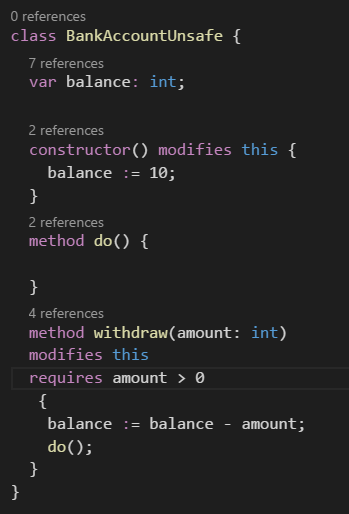
\includegraphics[width=1\textwidth]{img/codelensesClosed}
	\caption{Code Lenses used with Dafny}
	\label{fig:codelensesclosed}
\end{figure}

The first decision to be made was for which elements in the code codelenses should be displayed. The adeoff here is to  provide enough information to work comfortably with the codebase and not to clutter the workspace with codelenses. It was decided to display codelenses for classes, methods (including constructors) and fields, since they tend to have a wide scope in the codebases. \newline
A second consideration was which information should be displayed in the codelens. When codelenses are language specific and do not for instance stem from a plugin which displays code metrics are similar, usually references and usages of the element are displayed. Since this allows the programmer to gain a deeper understanding of control flow and regions affected by refactorings, it was decided to display this information also for the Dafny plugin. Codelenses also allow commands to be executed when clicked upon, a logical conclusion is to implement go to reference when a reference in a codelens is clicked.\newline

\begin{figure}[H]
	\centering
	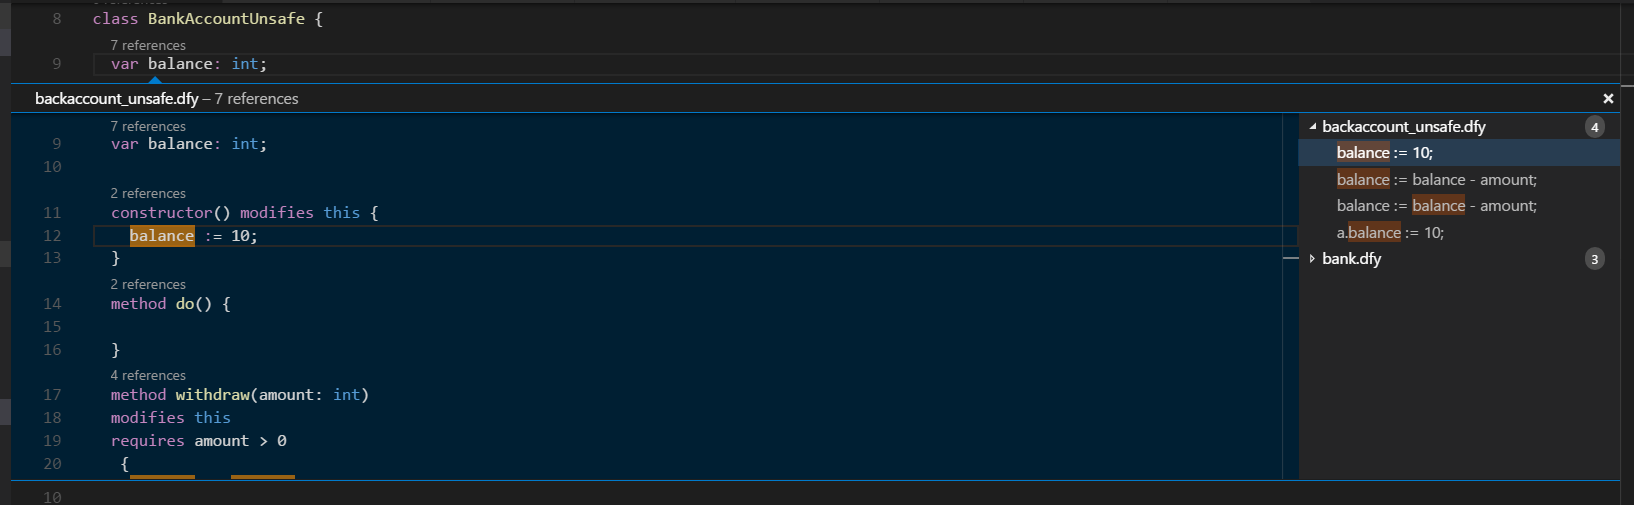
\includegraphics[width=1\textwidth]{img/codelensesExpanded}
	\caption{Expanded codelens showing the references to the field balance}
	\label{fig:codelensesexpanded}
\end{figure}

The only challenging aspect when implementing this feature is that references can't be determined via a simple text search, since different classes could have member with the same name. To only display unambiguous references, the search has to be done via the fully qualified domain name of the symbol. Since information about references is needed often, all references are determined by the DafnyServer and returned together with the symbolinformation to the symbolservice. This allows for simple processing in the language server itself and the references are updated in real time, since the symbolservice refreshes the symbols for a file when it is changed. Off course also the filepath belonging to the file in which the reference occurs is returned by the symbolservice. This is needed when a reference is a file external to the defining one and the go to reference command is invoked.\newline
When given locations of the references, it is possible to let visual studio code highlight them in the preview window which opens when a codelens is expanded. Visual studio code also groups references according to the filepath in the location, so the programmer gets to see a map of all references ordered by containing file to the right of preview window and can quickly navigating to them.











 \subsection{Code Completion} \label{codecompletion}
 

\subsection{Go to Definition} \label{gotodefinition}

\subsection{Rename Element} \label{renameelement}

\subsection{Quick Fixes} \label{quickfixes}